\chapter{Функция Грина оператора Лапласа, ее симметрия. Представление решения задачи Дирихле через функцию Грина. Метод отражений. Метод конформных отображений.}
\label{cha:17}

\section*{Функция Грина оператора Лапласа, ее симметрия.}

Рассмотрим фундаментальное решение оператора Лапласса:
$$ \triangle \varepsilon (x) = \delta (x) , \; \varepsilon (x) = 
\begin{cases}
	\displaystyle \frac{1}{2 \pi} \ln |\vec{x}|, \; \vec{x} \in \mathbb{R}^2\\
	\displaystyle - \frac{1}{4 \pi |\vec{x}|}, \; \vec{x} \in \mathbb{R}^3
\end{cases}$$

Рассмотрим задачу Дирихле: 
$\begin{cases}
	\triangle u = f (x) , x \in \Omega\\
	u|_{x \in \partial \Omega} = h(x)
\end{cases}$

\begin{definition}
	\red{Функция Грина} $ G(x, y) $ задачи Дирихле для области $ \Omega $ имеет вид:
	$$\begin{cases}
		\Delta_x G(x, y) = \delta(x - y), \; x \in \Omega \\
		G(x, y)|_{x \in \Omega} = 0
	\end{cases} \forall \; y \in \Omega$$
\end{definition}

\begin{definition}[\blue{эквивалентное определение функции Грина}]
	\red{Функция Грина} представляется в виде $ G(x,y) = \varepsilon(x - y) + g(x, y) $, где:
	$$
	\begin{cases}
		\Delta_x g(x, y) = \delta(x - y), \; x \in \Omega \\
		g(x, y)|_{x \in \Omega} = -\varepsilon(x - y)
	\end{cases} \; \forall \; y \in \Omega
	$$
\end{definition}\newpage

\begin{theorem}[\red{Симметрия функции Грина}]
	$G(x, y) = G(y, x)$
\end{theorem}
\begin{Proof}
	\begin{multicols}{2}
		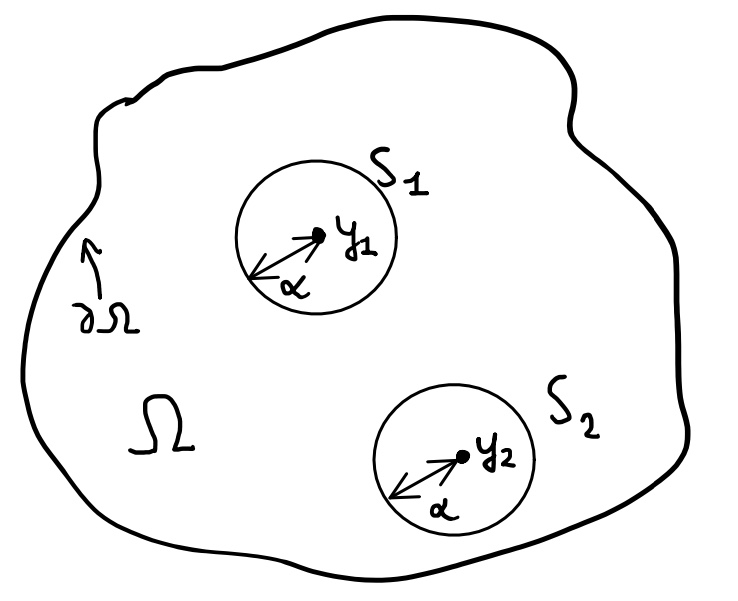
\includegraphics[scale=0.25]{cha17im1}
		\columnbreak
		$$\begin{gathered}
			\\
			\text{Рассмотрим две функции:}\\
			G_1 = G(x, y_1), \;  G_2 = G(x, y_2) \\ \\
			\text{Рассмотрим область:}\\
			\Omega_1 = \Omega \setminus (\left\{ {|x - y_1| < \alpha} \right\} \cup \left\{ {|x - y_2| < \alpha} \right\})
		\end{gathered}$$
	\end{multicols}

	Применим 2-ую формула Грина для $G_1$, $G_2$ в области $\Omega_1$:
	$$\begin{gathered}
		0 = \iint \limits_{\Omega_1} (G_1 \underbrace{\triangle_x G_2}_{ = 0} - G_2 \underbrace{\triangle_x G_1}_{ = 0}) d \vec{x} = 0 = \oint \limits_{\partial \Omega_1} \left(G_1 \frac{\partial G_2}{\partial n_x} - G_2 \frac{\partial G_1}{\partial n_x}\right) d \sigma = \\
		= \underbrace{\oint \limits_{\partial \Omega}\left(G_1 \frac{\partial G_2}{\partial n_x} - G_2 \frac{\partial G_1}{\partial n_x}\right) d \sigma}_{I_1} + \underbrace{\oint \limits_{S_1}\left(G_1 \frac{\partial G_2}{\partial n_x} - G_2 \frac{\partial G_1}{\partial n_x}\right) d \sigma}_{I_2} + \underbrace{\oint \limits_{S_2}\left(G_1 \frac{\partial G_2}{\partial n_x} - G_2 \frac{\partial G_1}{\partial n_x}\right) d \sigma }_{I_3}\\
		\left( S_1 \text{ и } S_2  \text{ - вырезанные окружности}\right)
	\end{gathered}$$

	$I_1 = 0$, т.к. $G_1$ и $G_2$ равны 0 на $\Omega$.

	Рассмотрим $I_2$:
	$$\begin{gathered} 
		\oint \limits_{S_1} \left(G(x, y_1) \frac{\partial}{\partial n_x} G(x, y_2) - G(x, y_2) \frac{\partial}{\partial n_x} G(x, y_1) d \sigma_x \right) = \\
		=\oint \limits_{S_1} (\varepsilon (x - y_1) + \underbrace{g(x, y_1)}_{\underset{\alpha \rightarrow 0}{\longrightarrow 0}}) \frac{\partial}{\partial n_x} G(x, y_2) - G(x, y_2) \frac{\partial}{\partial n_y} (\varepsilon (x - y_1) + \underbrace{g(x, y_1)}_{\underset{\alpha \rightarrow 0}{\longrightarrow 0}}) d \sigma_x \\
	\end{gathered}$$
	Сделаем замену: $|x - y_1| = \rho, \frac{\partial}{\partial n_x} = - \frac{\partial}{\partial \rho}$. Тогда при $\alpha \to 0$ интеграл стремится к:
	$$\begin{gathered} \int \limits_{0}^{2 \pi} ( \dfrac{1}{2 \pi} \ln \rho ( - \frac{\partial G_2}{\partial \rho} ) \rho) |_{\rho = \alpha} d \theta - \int \limits_{0}^{2 \pi} ( G_2 ( - \frac{1}{2 \pi \rho} ) \rho) |_{\rho = \alpha} d \theta  = \\
	= \underbrace{\alpha \ln \alpha \frac{1}{2 \pi} \int \limits_{0}^{2 \pi}(- \frac{\partial G_2}{\partial \rho}) |_{\rho = \alpha} d \theta}_{\underset{\alpha \rightarrow 0}{\longrightarrow 0}} + \frac{1}{2 \pi} \int \limits_{0}^{2 \pi} G_2 |_{\rho = \alpha} d \theta
	 \end{gathered}$$ 

	$$ = \Big|\text{по теореме о среднем}\Big| =  G(x^*, y_2) |_{x^* \in S_1} \underbrace{\frac{1}{2 \pi} \int \limits_{0}^{2 \pi} d \theta}_{=1} \xrightarrow[\alpha \to 0]{} G(y_1, y_2) $$

	Для $\oint \limits_{S_2}$ все аналогично, только меняем местами $ G_1 $ и $ G_2 $. Тогда $\oint \limits_{S_2} \underset{\alpha \rightarrow 0}{\longrightarrow} G(y_2, y_1)$.
	
	В итоге получаем, что $G(y_1, y_2) - G(y_2, y_1) = 0$. Т.к. $ y_1, y_2 $ -- произвольные точки из $\Omega$, то $G(y_1, y_2) = G(y_2, y_1) \; \forall \; y_1, y_2 \in \Omega.$

\end{Proof}

\section*{Представление решения задачи Дирихле через функцию Грина.}

Имеем задачу Дирихле: 
$\begin{cases}
	\triangle u = f (x) , x \in \Omega\\
	u|_{x \in \partial \Omega} = h(x)
\end{cases}$\\

Воспользуемся 2-ой формулой Грина для $ u(y), G(x, y): $
$$\begin{gathered} 
	\iint\limits_{\Omega}\left(u(y) \underbrace{\triangle_y G(x,y)}_{=\delta (y-x)} - G(x,y)\underbrace{\triangle_y u(y)}_{=f(y)}\right)dy = \oint\limits_{\partial \Omega}\left(\underbrace{u(y)}_{=h(y)}\dfrac{\partial G(x,y)}{\partial n_y} - \underbrace{G(x,y)}_{=0}\dfrac{\partial u(y)}{\partial n_y}\right)d\sigma \\
	\iint\limits_{\Omega}\underbrace{u(y)\delta(y - x)}_{=u(x)\delta(y-x)}dy =  u(x) \underbrace{\iint\limits_{\Omega}\delta(y - x)dy}_{=1} = u(x)
\end{gathered}$$
Тогда получаем формулу:
$$u(x) = \displaystyle \iint\limits_{\Omega} G(x,y)f(y)dy + \oint\limits_{\partial \Omega}h(y)\dfrac{\partial G(x,y)}{\partial n_y}d\sigma_y$$

\section*{Метод отражений.}

\begin{center}
	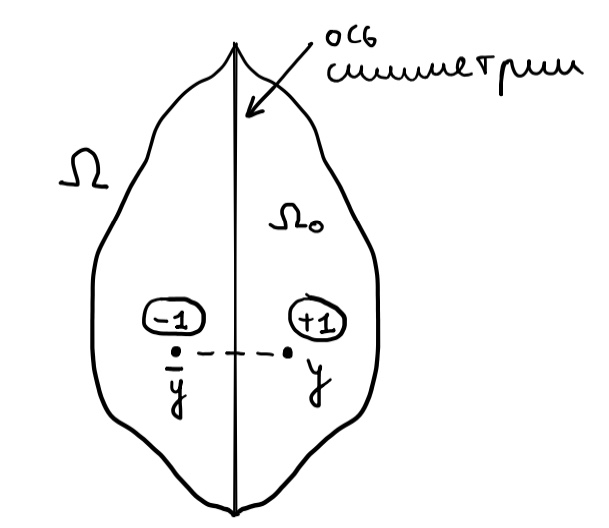
\includegraphics[scale=0.4]{cha17im2}
\end{center}
	
Воспользуемся тем, что одной из физических интерпретаций функции Грина задачи Дирихле в области $ \Omega_0 $ является потенциал поля, создаваемого в точке $ x \in \Omega_0 $ точечным зарядом величины $ q = \dfrac{1}{4\pi} $, расположенным в точке $ y \in \Omega_0 $, если граница $ \partial \Omega_0 $ области $ \Omega_0 $ является заземленной идеально проводящей поверхностью.

Предположим, что вне области $ \Omega_0 $ можно расположить фиктивные электрические заряды таким образом, чтобы суммарный потенциал поля, создаваемого зарядом $ q = \dfrac{1}{4\pi} $, расположенным в точке $ y \in \Omega_0 $, и этими фиктивными зарядами, на границе $ \partial \Omega_0 $ обращался в нуль. Такие фиктивные заряды называются электростатическими изображениями заряда, помещенного в точку $ y \in \Omega_0 $. Потенциал поля, порожденного зарядами, находящимися вне области, представляет собой гармоническую внутри области $ \Omega_0 $ функцию, то есть искомое гармоническое слагаемое в функции Грина.

Тогда в условиях вышеописанной задачи потенциал есть $ u(x) = \varepsilon(x - y) + g(x,y) = G(x, y), \; g(x, y)$ -- гармоническая. $ G_0(x, y) $ -- функция Грина для половинки, тогда
$$\begin{cases}
	\Delta_x G_0(x, y) = \delta(x - y), \; x \in \Omega_0 \\
	G_0(x, y)|_{x \in \Omega_0} = 0
\end{cases} \; \forall y \in \Omega_0$$
\begin{theorem}[]\label{lec:17/the:1}
	$ G_0(x, y) = G(x, y) - G(x, \bar{y}) $.
\end{theorem}
\begin{Proof}
	\begin{enumerate}
		\item 
			\begin{itemize}
				\item[$\bullet$]
					$G_0(x, y)|_{x \in \Omega} = 0, \text{ т.к. } G(x, y)|_{x \in \Omega} = 0$
				\item[$\bullet$]
					$G_0(x, y)|_{\text{на } l} = 0, \text{ т.к. суммарный потенциал поля обращается }\text{в нуль на } l$
			\end{itemize}
			Значит $ G_0(x, y)|_{x \in \Omega_0} = 0 $.
		\item 
			$ \triangle_x G_0(x, y) = \delta(x-y) $, т.к.:
			$$\triangle_x G_0(x, y) = \triangle_x G(x, y) - \triangle_x G(x, \bar{y}) = \delta(x-y) - \underbrace{\delta(x-\bar{y})}_{= 0 \text{ в } \Omega_0 \; \left(\bar{y} \not\in \Omega_0\right)}$$
	\end{enumerate}
	Таким образом, $ G_0(x, y) = G(x, y) - G(x, \bar{y}). $
\end{Proof}

\section*{Метод конформных отображений.}

\begin{center}
		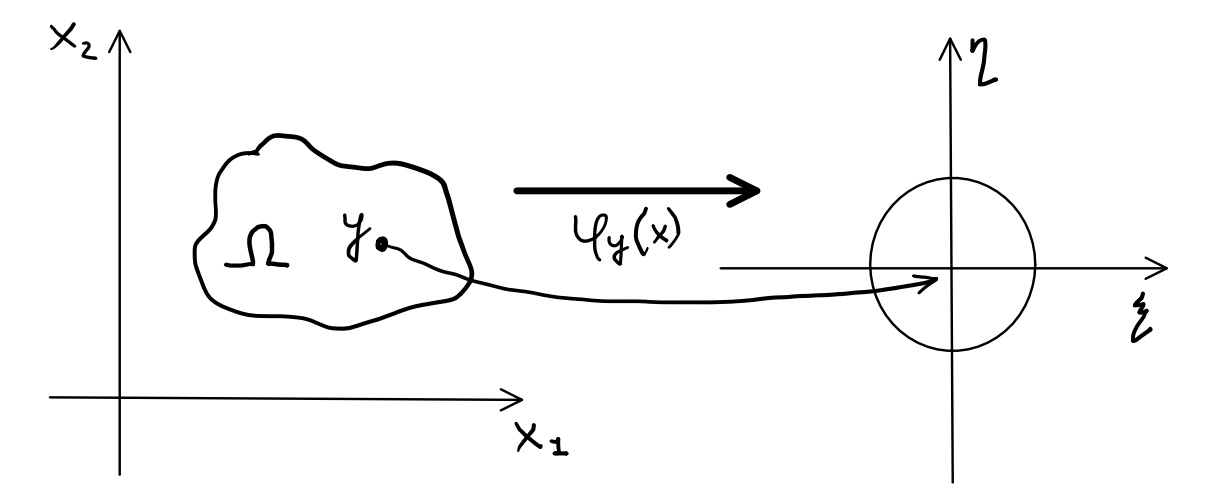
\includegraphics[scale=0.4]{cha17im3}
		
		$ \varphi(x): \; \mathbb{R}^2 \longrightarrow \mathbb{C} $
		
		$ \varphi(x) = \xi(x_1, x_2) + i \eta(x_1, x_2) $
\end{center}

\begin{definition}
	$ \varphi(x) $ -- \red{конформное отображение}, если $ \varphi(x) $ есть аналитическая функция ($ \mathbb{C} \text{ - дифференцируема, } \varphi'(x) \neq 0$).
\end{definition}

\begin{definition}
	$ \varphi(x) $ - \red{аналитическая функция} $\Leftrightarrow$ выполнены условия \textit{Коши - Римана:} 
	$$\begin{cases}
		\dfrac{\partial \xi}{\partial x_1} = \dfrac{\partial \eta}{\partial x_2} \\
		-\dfrac{\partial \xi}{\partial x_2} = \dfrac{\partial \eta}{\partial x_1}
	\end{cases}$$
\end{definition}

Функция $ \varphi_y(x) $ -- аналитическая, $ \frac{\partial \varphi_y(x)}{\partial x} \neq 0. $ Пусть $ \varphi_y(x) $ такая, что удовлетворяет условиям:
$$\begin{gathered} 
	x \to \varphi_y(x), \; y \to 0 \\
	\Omega \to |\varphi_y| < 1, \; \partial\Omega \to |\varphi_y| = 1
\end{gathered}$$
Получаем, что $G(x, y) \to G(\varphi_y, 0)$.
$$\begin{gathered} 
	G(\varphi_y, 0) = \varepsilon(\varphi_y - 0) = \varepsilon(\varphi_y) = \dfrac{1}{2\pi}\log|\varphi_y| \\
	\triangle \varepsilon(\varphi_y) = \xi_{\varphi_y\varphi_y} + \eta_{\varphi_y\varphi_y} = \delta(\varphi_y)
\end{gathered}$$
Значит:
$\begin{cases}
	\displaystyle \Delta_{\varphi_y} G(\varphi_y, 0) = \delta(\varphi_y - 0), |\varphi_y| < 1 \\
	\displaystyle G(\varphi_y, 0)|_{|\varphi_y| = 1} = 0
\end{cases}$

\begin{clair}
	$ G(x, y) = \dfrac{1}{2\pi} \ln|\varphi_y(x)|$.
\end{clair}
\begin{Proof}
	\begin{enumerate}
		\item 
			$ \displaystyle \partial\Omega \to |\varphi_y| = 1 \; \Rightarrow \; G(x, y)|_{x \in \partial \Omega} = \dfrac{1}{2\pi} \ln|\varphi_y(x)| \Big|_{|\varphi_y| = 1} = \dfrac{1}{2\pi} \ln1 = 0$.
		\item 
			Рассмотрим случай $x \neq y$:

			$\ln z = \ln|z| + iArg(z) $ - аналитическая при $ z \neq 0$, тогда $\varphi_y(x) $ -- аналитическая при $ \varphi_y(x) \not = 0$.
			$$G(x, y) = \dfrac{1}{2\pi}\ln|\varphi_y(x)| = \dfrac{1}{2\pi} \Re e(\ln(\varphi_y(x))) \text{ - гармоническая при } \\
			x \not = y.$$
			Тогда $\triangle_x G(x,y) = 0$ при $x \not = y$.
		\item 
			Рассмотрим случай $x \to y$.
			$$\begin{gathered} 
			\varphi_y(x) = \underbrace{\varphi_y(y)}_{= 0} + \underbrace{\dfrac{d \varphi_y(x)}{dx}\Big|_{x = y}}_{\neq 0}\cdot(x - y) + \underbrace{\alpha(x,t)}_{\underset{x \rightarrow y}{\longrightarrow} 0}(x - y)
			\end{gathered}$$
			Тогда 
			$$\begin{gathered} 
			G(x, y) = \dfrac{1}{2\pi}\ln|\varphi_y(x)| = \dfrac{1}{2\pi}\ln\left|\dfrac{d \varphi_y(x)}{dx}\Big|_{x = y}(x - y) + \alpha(x,t)(x - y)\right| = \\
			= \dfrac{1}{2\pi} \ln \left(|x - y|\left|\left.\dfrac{d \varphi_y(x)}{dx}\right|_{x = y} + \alpha(x,t)\right|\right) = \\
			= \underbrace{\dfrac{1}{2\pi} \ln|x - y|}_{=\epsilon (x-y)} + \dfrac{1}{2\pi} \ln\Big|\underbrace{\dfrac{d \varphi_y(x)}{dx}|_{x = y}}_{\not = 0} + \underbrace{\alpha(x,t)}_{\to 0}\Big| = \\
			= \varepsilon(x - y) + g(x, y), \; |g(x, y)| < C \; x \longrightarrow y.
			\end{gathered}$$
			Отсюда следует, что 
			$$\begin{gathered} 
			\triangle_x G(x, y) = \triangle_x (\varepsilon(x - y) + g(x, y)) = \delta(x - y) + \triangle_x g(x, y) = \\
			= \underbrace{\delta(x - y)}_{= 0, \text{ при } x \neq y} + \triangle_x g(x, y)
			\end{gathered}$$
			$$\begin{cases}
				\triangle_x g(x, y) = 0, \; x \neq y \\
				|g(x,y)| < C, \; x \to y
			\end{cases} \Rightarrow \;  \triangle_x g(x, y) = 0$$
			Получаем, что 
			$\displaystyle \triangle_x G(x, y) = \delta(x - y)$.
	\end{enumerate}
\end{Proof}












